\documentclass[notes,10pt, aspectratio=169]{beamer}

\usepackage{pgfpages}
% These slides also contain speaker notes. You can print just the slides,
% just the notes, or both, depending on the setting below. Comment out the want
% you want.
\setbeameroption{hide notes} % Only slide
%\setbeameroption{show only notes} % Only notes
%\setbeameroption{show notes on second screen=right} % Both
\usepackage{colortbl}
\usepackage{helvet}
\usepackage[default]{lato}
\usepackage{array}
\usepackage{eurosym}
\usepackage{setspace}
\usepackage{animate}
\usepackage{multicol}
\usepackage{breqn}
\usepackage{subcaption}
\usepackage{caption}
\captionsetup{font=scriptsize, justification=raggedright,singlelinecheck=false}
\usepackage[export]{adjustbox}
\usepackage[scale=2]{ccicons}
\usepackage{tikz}
\newenvironment{wideitemize}{\itemize\addtolength{\itemsep}{10pt}}{\enditemize}
\usepackage{natbib}

\usepackage{tikz}
\usepackage{verbatim}
\setbeamertemplate{note page}{\pagecolor{yellow!5}\insertnote}
\usepackage{amsmath}
%\usepackage{mathpazo}
\usepackage{hyperref}
\usepackage{lipsum}
\usepackage{multimedia}
\usepackage{multirow}
\usepackage{graphicx}
\usepackage{dcolumn}
\usepackage{bbm}
\newcolumntype{d}[0]{D{.}{.}{5}}

\usepackage{changepage}
\usepackage{appendixnumberbeamer}
% \newcommand{\beginbackup}{
%   \newcounter{framenumbervorappendix}
%   \setcounter{framenumbervorappendix}{\value{framenumber}}
%   \setbeamertemplate{footline}
%   {
%      \leavevmode%
%      \hline
%      box{%
%       \begin{beamercolorbox}[wd=\paperwidth,ht=2.25ex,dp=1ex,right]{footlinecolor}%
% %         \insertframenumber  \hspace*{2ex} 
%       \end{beamercolorbox}}%
%      \vskip0pt%
%   }
%  }

 \setbeamertemplate{footline}{
    \hbox{%
    \begin{beamercolorbox}[wd=\paperwidth,ht=3ex,dp=1.5ex,leftskip=2ex,rightskip=2ex]{page footer}%
        %\usebeamerfont{title in head/foot}%
        %\insertshorttitle \hfill
        %\insertsection \hfill
        %\tableofcontents[currentsection] \hfill
        \insertsectionnavigationhorizontal{0.7\paperwidth}{}{} \hfill 
        \insertframenumber{} / \inserttotalframenumber
    \end{beamercolorbox}}%
}
\newcommand{\backupend}{
   \addtocounter{framenumbervorappendix}{-\value{framenumber}}
   \addtocounter{framenumber}{\value{framenumbervorappendix}} 
}

\useinnertheme[shadow]{rounded}
\setbeamercolor{block title example}{fg=black,bg=orange!50!white}
\setbeamercolor{block body example}{fg=black, bg=orange!30!white}
\setbeamercolor{block title alert}{fg=black,bg=green!50!white}
\setbeamercolor{block body alert}{fg=black, bg=green!30!white}
\setbeamercolor{block title}{use=structure,fg=structure.fg,bg=structure.fg!20!bg}
\setbeamercolor{block body}{parent=normal text,use=block title,bg=block title.bg!50!bg}

\newcommand\independent{\protect\mathpalette{\protect\independenT}{\perp}}
\def\independenT#1#2{\mathrel{\rlap{$#1#2$}\mkern2mu{#1#2}}}

\usepackage{graphicx}
\usepackage[space]{grffile}
\usepackage{booktabs}

% These are my colors -- there are many like them, but these ones are mine.
\definecolor{blue}{RGB}{0,114,178}
\definecolor{red}{RGB}{213,94,0}
\definecolor{yellow}{RGB}{240,228,66}
\definecolor{green}{RGB}{0,158,115}

\setbeamercolor{section in head/foot}{fg=blue}


\hypersetup{
  colorlinks=false,
  linkbordercolor = {white},
  linkcolor = {blue}
}


%% I use a beige off white for my background
\definecolor{MyBackground}{RGB}{255,253,218}

%% Uncomment this if you want to change the background color to something else
%\setbeamercolor{background canvas}{bg=MyBackground}

%% Change the bg color to adjust your transition slide background color!
\newenvironment{transitionframe}{
  \setbeamercolor{background canvas}{bg=yellow}
  \begin{frame}}{
    \end{frame}
}

\setbeamercolor{frametitle}{fg=blue}
\setbeamercolor{title}{fg=black}
%\setbeamertemplate{footline}[frame number]
\setbeamertemplate{navigation symbols}{} 
\setbeamertemplate{itemize items}{-}
\setbeamercolor{itemize item}{fg=blue}
\setbeamercolor{itemize subitem}{fg=blue}
\setbeamercolor{enumerate item}{fg=blue}
\setbeamercolor{enumerate subitem}{fg=blue}
\setbeamercolor{button}{bg=white,fg=blue,}



% If you like road maps, rather than having clutter at the top, have a roadmap show up at the end of each section 
% (and after your introduction)
% Uncomment this is if you want the roadmap!
% \AtBeginSection[]
% {
%    \begin{frame}
%        \frametitle{Roadmap of Talk}
%        \tableofcontents[currentsection]
%    \end{frame}
% }
\setbeamercolor{section in toc}{fg=blue}
\setbeamercolor{subsection in toc}{fg=red}
%\setbeamersize{text margin left=1em,text margin right=1em} 
\setbeamersize{text margin left=0.7cm,text margin right=0.7cm} 


\title[]{\textcolor{blue}{Lecture 9:\\An Introduction to Instrumental Variables}}
\author{25117 - Econometrics}
\institute[shortinst]{Universitat Pompeu Fabra}

\date{November 18th, 2024}

\begin{document}

\begin{frame}[plain]
\maketitle
\end{frame}



\begin{frame}{What we learned in the last lesson}
\item Statistical studies are evaluated by asking whether the analysis is internally and externally valid.\\[1em]
\begin{itemize}
    \item A study is internally valid if the statistical inferences about causal effects are valid for the population being studied. In regression estimation of causal effects, there are two main types of threats to internal validity:
    \begin{itemize}
        \item First, OLS estimators are biased and inconsistent if the regressors and error terms are correlated.
        \item Second, confidence intervals and hypothesis tests are not valid when the standard errors are incorrect.
    \end{itemize}\\[1em]
    \item A study is externally valid if its inferences and conclusions can be generalized from the population and setting studied to other populations and settings.
\end{itemize} 
\end{frame}


\begin{frame}{Instrumental Variables}
Consider the following regression model:
\begin{equation*}
    Y_i = \beta_0 + \beta_1 X_i + u_i
\end{equation*}
\begin{itemize}
    \item OVB,  Simultaneous causality bias, Errors-in-variables bias... all three result in $\mathbb{E}(u\mid X)\neq0$\\[1em]
    \item Instrumental variables regression can eliminate bias when $\mathbb{E}(u\mid X)\neq0$, using an instrumental variable (IV), $Z$.\\[1em]
    \item Intuitively, IV regression breaks $X$ into two parts:
    \begin{enumerate}
        \item an \textit{endogenous} part that might be correlated with $u$, and 
        \item an \textit{exogenous}  part that is not. 
    \end{enumerate}\\[1em]
By isolating the part that is not correlated with $u$, it is possible to estimate $\beta_1$
\end{itemize}
\end{frame}



\begin{frame}{Instrumental Variables}
For an instrumental variable (an “instrument”) Z to be valid, it must satisfy two conditions:
\begin{enumerate}
    \item \textbf{Instrument relevance:} $Z$ is a strong determinant of $X$ ($corr(Z, X)\neq 0$)
    \item \textbf{Instrument exogeneity (exclusion restriction):} $Z$ is unrelated to $u$ ($corr(Z, u) = 0$)
\end{enumerate}

\begin{center}
\begin{figure}
    \resizebox{.9\linewidth}{!}{%

\tikzset{every picture/.style={line width=0.75pt}} %set default line width to 0.75pt        

\begin{tikzpicture}[x=0.75pt,y=0.75pt,yscale=-1,xscale=1]
%uncomment if require: \path (0,292); %set diagram left start at 0, and has height of 292

%Shape: Ellipse [id:dp6518310746416693] 
\draw   (187.23,223.93) .. controls (187.23,206.77) and (201.01,192.85) .. (218,192.85) .. controls (234.99,192.85) and (248.77,206.77) .. (248.77,223.93) .. controls (248.77,241.09) and (234.99,255) .. (218,255) .. controls (201.01,255) and (187.23,241.09) .. (187.23,223.93) -- cycle ;
%Shape: Ellipse [id:dp21717165537664984] 
\draw   (556.46,222.68) .. controls (556.46,205.52) and (570.24,191.61) .. (587.23,191.61) .. controls (604.22,191.61) and (618,205.52) .. (618,222.68) .. controls (618,239.85) and (604.22,253.76) .. (587.23,253.76) .. controls (570.24,253.76) and (556.46,239.85) .. (556.46,222.68) -- cycle ;
%Shape: Ellipse [id:dp6180865660156953] 
\draw   (358.31,66.07) .. controls (358.31,48.91) and (372.08,35) .. (389.08,35) .. controls (406.07,35) and (419.85,48.91) .. (419.85,66.07) .. controls (419.85,83.23) and (406.07,97.15) .. (389.08,97.15) .. controls (372.08,97.15) and (358.31,83.23) .. (358.31,66.07) -- cycle ;
%Shape: Ellipse [id:dp049861641718563554] 
\draw  [color={rgb, 255:red, 11; green, 8; blue, 234 }  ,draw opacity=1 ] (42,84.72) .. controls (42,67.56) and (55.78,53.64) .. (72.77,53.64) .. controls (89.76,53.64) and (103.54,67.56) .. (103.54,84.72) .. controls (103.54,101.88) and (89.76,115.79) .. (72.77,115.79) .. controls (55.78,115.79) and (42,101.88) .. (42,84.72) -- cycle ;
%Straight Lines [id:da038069870660455196] 
\draw [color={rgb, 255:red, 6; green, 20; blue, 244 }  ,draw opacity=1 ] [dash pattern={on 4.5pt off 4.5pt}]  (94.92,107.09) -- (192.48,203.18) ;
\draw [shift={(194.62,205.28)}, rotate = 224.57] [fill={rgb, 255:red, 6; green, 20; blue, 244 }  ,fill opacity=1 ][line width=0.08]  [draw opacity=0] (8.93,-4.29) -- (0,0) -- (8.93,4.29) -- cycle    ;
%Straight Lines [id:da7311874040313404] 
\draw [color={rgb, 255:red, 244; green, 6; blue, 31 }  ,draw opacity=1 ] [dash pattern={on 4.5pt off 4.5pt}]  (361.09,88.06) -- (243.53,203.18) ;
\draw [shift={(241.38,205.28)}, rotate = 315.6] [fill={rgb, 255:red, 244; green, 6; blue, 31 }  ,fill opacity=1 ][line width=0.08]  [draw opacity=0] (8.93,-4.29) -- (0,0) -- (8.93,4.29) -- cycle    ;
\draw [shift={(363.23,85.96)}, rotate = 135.6] [fill={rgb, 255:red, 244; green, 6; blue, 31 }  ,fill opacity=1 ][line width=0.08]  [draw opacity=0] (8.93,-4.29) -- (0,0) -- (8.93,4.29) -- cycle    ;
%Straight Lines [id:da7673731200325982] 
\draw [color={rgb, 255:red, 126; green, 211; blue, 33 }  ,draw opacity=1 ]   (248.77,223.93) -- (553.46,222.7) ;
\draw [shift={(556.46,222.68)}, rotate = 179.77] [fill={rgb, 255:red, 126; green, 211; blue, 33 }  ,fill opacity=1 ][line width=0.08]  [draw opacity=0] (8.93,-4.29) -- (0,0) -- (8.93,4.29) -- cycle    ;
%Straight Lines [id:da44429091772583584] 
\draw [color={rgb, 255:red, 61; green, 222; blue, 2 }  ,draw opacity=1 ]   (414,84) -- (562.71,199.71) ;
\draw [shift={(565.08,201.55)}, rotate = 217.89] [fill={rgb, 255:red, 61; green, 222; blue, 2 }  ,fill opacity=1 ][line width=0.08]  [draw opacity=0] (8.93,-4.29) -- (0,0) -- (8.93,4.29) -- cycle    ;
%Curve Lines [id:da5510041670949384] 
\draw  [dash pattern={on 0.84pt off 2.51pt}]  (328,124) .. controls (400.64,233.45) and (560.39,197.37) .. (530.47,89.63) ;
\draw [shift={(530,88)}, rotate = 73.64] [color={rgb, 255:red, 0; green, 0; blue, 0 }  ][line width=0.75]    (10.93,-3.29) .. controls (6.95,-1.4) and (3.31,-0.3) .. (0,0) .. controls (3.31,0.3) and (6.95,1.4) .. (10.93,3.29)   ;
%Curve Lines [id:da9877608396858246] 
\draw  [dash pattern={on 0.84pt off 2.51pt}]  (463,120) .. controls (457.06,122.97) and (548.15,150.44) .. (530.57,89.86) ;
\draw [shift={(530,88)}, rotate = 72.39] [color={rgb, 255:red, 0; green, 0; blue, 0 }  ][line width=0.75]    (10.93,-3.29) .. controls (6.95,-1.4) and (3.31,-0.3) .. (0,0) .. controls (3.31,0.3) and (6.95,1.4) .. (10.93,3.29)   ;
%Curve Lines [id:da31587639785238864] 
\draw  [dash pattern={on 0.84pt off 2.51pt}]  (80.14,51.79) .. controls (98.88,16.95) and (120.26,40.2) .. (133,50) ;
\draw [shift={(79,54)}, rotate = 296.57] [color={rgb, 255:red, 0; green, 0; blue, 0 }  ][line width=0.75]    (10.93,-3.29) .. controls (6.95,-1.4) and (3.31,-0.3) .. (0,0) .. controls (3.31,0.3) and (6.95,1.4) .. (10.93,3.29)   ;

% Text Node
\draw (66,75) node [anchor=north west][inner sep=0.75pt]  [color={rgb, 255:red, 13; green, 16; blue, 187 }  ,opacity=1 ] [align=left] {$Z$};
% Text Node
\draw (212,217.29) node [anchor=north west][inner sep=0.75pt]   [align=left] {$X$};
% Text Node
\draw (580.23,214.05) node [anchor=north west][inner sep=0.75pt]   [align=left] {$Y$};
% Text Node
\draw (383,60) node [anchor=north west][inner sep=0.75pt]   [align=left] {$u$};
% Text Node
\draw (489,69) node [anchor=north west][inner sep=0.75pt]   [align=left] {$\mathbb{E}(u\mid X)\neq0$};
% Text Node
\draw (113,53) node [anchor=north west][inner sep=0.75pt]   [align=left] {Instrumental Variable (IV)};


\end{tikzpicture}
}
\end{figure}
\end{center}

\end{frame}




\begin{frame}{Two Stages Least Squares (2SLS)}
Assume that $Z$ satifies both conditions. Then the 2SLS estimator of $\beta_1$ is obtained by
\begin{itemize}
    \item \textbf{First Stage ---} Regress $X_i$ on $Z_i$ (including the intercept), and obtain the predicted values $\hat{X}_i$.
    \item \textbf{Second Stage ---} Regress $Y_i$ on $\hat{X}_i$ (including the intercept), the coefficient on $\hat{X}_i$ is the 2SLS estimator $\hat{\beta}_1^{2SLS}$
\end{itemize}\\[.5em]
Formally, suppose that $Z$ satisfies both conditions. As a first step, suppose that we use it as a proxy for $X$. The reduced-form estimator, $\beta_1^{RF}$, reads
\begin{eqnarray*}
    & \beta_1^{RF} = \frac{cov(Z_i, Y_i)}{var(Z_i)}=\frac{cov(Z_i, [\beta_0 + \beta_1 X_i + u_i])}{var(Z_i)}=\beta_1\frac{cov(Z_i, X_i)}{var(Z_i)}\\
    &\Rightarrow \beta_1 = \frac{cov(Z_i, Y_i)}{var(Z_i)}/\frac{cov(Z_i, X_i)}{var(Z_i)} = \frac{cov(Z_i, Y_i)}{cov(Z_i, X_i)}
\end{eqnarray*}
The IV estimator (replacing population covariances with the sample covariances) is a consistent estimator of $\beta_1$:
 \begin{eqnarray*}
    &\hat{\beta}_1^{2SLS}= \frac{s_{ZY}}{s_{ZX}} \overset{p}{\to}  \frac{cov(Z_i, Y_i)}{cov(Z_i, X_i)} = \beta_1 \text{~~~~~~~~~}\Biggl(\text{Note that~} \hat{\beta}_1^{OLS}= \frac{s_{XY}}{s_{XX}} \Biggr)
\end{eqnarray*}

\end{frame}

\begin{frame}{Two Stages Least Squares (2SLS)}
For another way to see it, consider the system of reduced-form equations:
\begin{eqnarray*}
    & X_i &= \pi_0 + \pi_1 Z_i + v_i\\
    & Y_i &= \gamma_0 + \gamma_1 Z_i + w_i
\end{eqnarray*}
Because $Z$ is exogenous, $Z$ is uncorrelated with both $v_i$ and $w_i$.\\[1em]
\underline{\textbf{The idea:}} An exogenous unit change in $Z$ results in a change in $X$ by $\pi_1$ units and a change in $Y$ by $\gamma_1$ units.\\[1em]

Thus an exogenous change in  $X$ by $\pi_1$ is associated with an exogenous change in $Y$ by $\gamma_1$ units.\\[1em]

So the effect on $Y$ of an exogenous change in $X$ is $\beta_1^{2SLS} = \gamma_1/\pi_1$
\end{frame}

\begin{frame}{A Buttery Example}
IV regressions were first developed in 1928 by Philip G. Wright to estimate supply and demand elasticities for agricultural goods,in particular, butter.\\[1em]

Consider the following demand equation:
\begin{equation*}
    ln(Q^{butter}_i) = \beta_0 + \beta_1 ln(P^{butter}_i)+ u_i
\end{equation*}
Here, $\beta_1$ captures the price-elasticity of butter, i.e., the percentage change in quantities due to a 1\% change in price.\\[1em]

\textbf{\underline{Problem:}} The OLS regression of $ln(Q^{butter}_i)$ on $ln(P^{butter}_i)$ suffers from simultaneity (reverse causality) bias.\\[1em]

Because prices, $ln(P^{butter}_i)$, are simultaneously determined in equilibrium by the interplay of supply and demand, $\beta_1$ was unlikely to capture neither the supply or demand elasticity of butter.

\end{frame}


\begin{frame}{A Buttery Example}
 \begin{columns}
\begin{column}{0.35\textwidth}
    \begin{itemize}
        \item In every period, prices are determined in equilibrium by the simultaneous movements of supply and demand 
        \item The equilibrium is determined by the intersection of the demand curve $D_k$ and supply curve $S_k$  
    \end{itemize}
\end{column}
\begin{column}{0.7\textwidth}
\begin{figure}
  \centering
         \vspace{-1mm}
        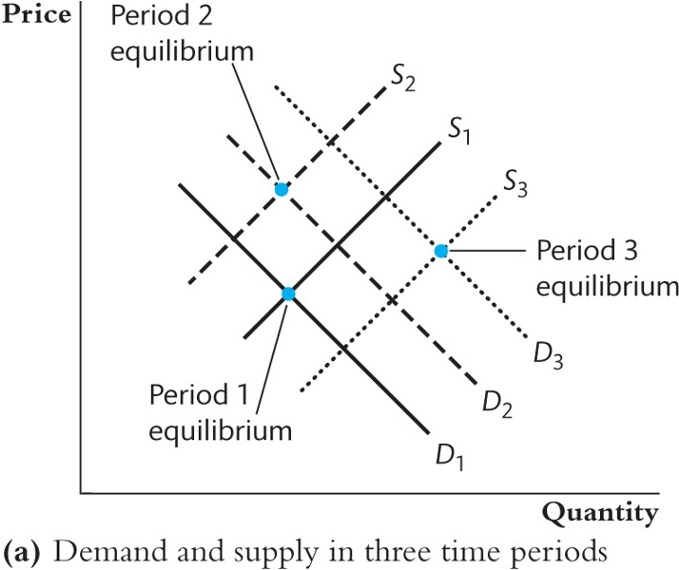
\includegraphics[scale=.35]{images/butter1.jpg}
\end{figure}
\end{column}
\end{columns}
\end{frame}

\begin{frame}{A Buttery Example}
 \begin{columns}
\begin{column}{0.35\textwidth}
    \begin{itemize}
        \item As a result, the set of $\{Price_k, Quantity_k\}$ is not informative about the specific demand and supply elasticities (i.e., the curves' slopes)
        \item In this example, demand and supply elasticities could be anything, from perfectly elastic (a small change in $P$ is associated with a high change in $Q$) to completely inelastic (a high change in $P$ is associated with a little change in $Q$).
    \end{itemize}
\end{column}
\begin{column}{0.7\textwidth}
\begin{figure}
  \centering
         \vspace{-1mm}
        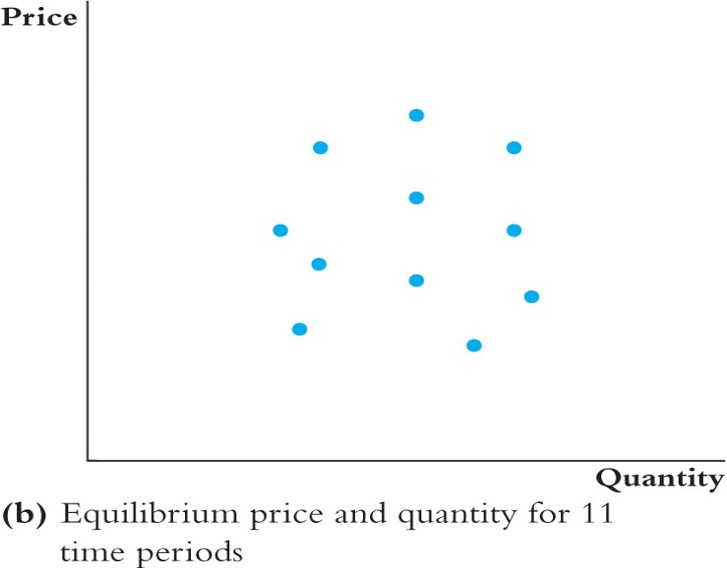
\includegraphics[scale=.35]{images/butter2.jpg}
\end{figure}
\end{column}
\end{columns}
\end{frame}

\begin{frame}{A Buttery Example}
 \begin{columns}
\begin{column}{0.35\textwidth}
    \begin{itemize}
        \item To determine the elasticity of demand, we need an IV that would shift only supply curves while leaving demand curves unchanged.
        \item What could be such an instrument?
    \end{itemize}
\end{column}
\begin{column}{0.7\textwidth}
\begin{figure}
  \centering
         \vspace{-1mm}
        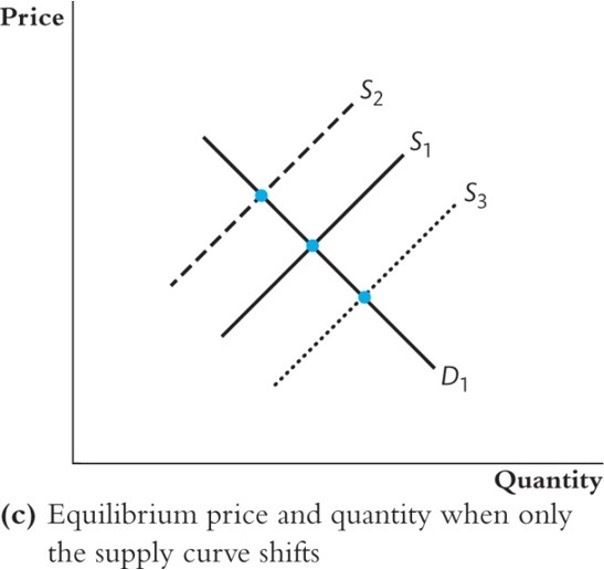
\includegraphics[scale=.35]{images/butter3.jpg}
\end{figure}
\end{column}
\end{columns}
\end{frame}

\begin{frame}{A Buttery Example}
A potential IV for the butter prices to estimate the demand elasticity for butter could be drought shocks to dairy regions ($Z$).\\[1em]
It is a plausibly revelant IV: below-average rainfall in a dairy region  ($Z$) could impair grazing and thus reduce butter production at a given price, shifting the supply curve to the left and increasing the equilibrium price  ($X$)\\[1em]
Drought shocks are also plausibly unrelated to the quantities of butter demanded  ($Y$)... except through the price increase ($X$)!\\[1em]
Can you think of an instrument to estimate the supply elasticity of butter? In the California Schools example, what could be an instrument for the share of subsidized meals?
\end{frame}

\begin{frame}{Large-Sample properties}
\begin{itemize}
    \item As $n\rightarrow\infty$, $\hat{\beta}_1^{2SLS}\sim\mathcal{N}(\beta_1, \sigma^2_{\hat{\beta}_1})$ where $\sigma^2_{\hat{\beta}_1}=\frac{1}{n}\frac{var(Zi-\mu_Z)u_i}{[cov(Z_i, X_i)]^2}$
    \item Statistical inference proceeds in the usual way.
    \item The justification is (as usual) based on large samples
    \item This all assumes that the instruments are valid -- we’ll discuss what happens if they aren’t valid shortly.
    \item However, the OLS standard errors from the second stage regression aren’t right because they do not account for the estimation in the first stage
    \item Instead, use a single specialized command that computes the 2SLS estimator and the correct SEs.
    \item As usual, use heteroskedasticity-robust SEs
\end{itemize}
\end{frame}

\begin{frame}{The General  IV  Regression Model }
We can extend the simple IV framework to multiple endogenous regressors ($X$s), exogenous regressors or control variables ($W$s), and exogenous instruments ($Z$s).\\[1em]
We say the coefficients $\beta_1, \dots, \beta_k$ are
\begin{itemize}
    \item \textbf{underidentified} if there are more regressors than instruments ($m<k)$.
    \item \textbf{exactly identified} if there are as many regressors as instruments ($m=k)$.
    \item \textbf{overidentified} if there are less regressors than instruments ($m>k)$.
\end{itemize}\\[1em]
E.g., with a single endogenous regressor:
\begin{equation*}
    Y_i = \beta_0 + \beta_1 X_{1i} + \beta_2 W_{1i} + \dots + \beta_{r+1} W_{ri} + u_i
\end{equation*}
and $m$ instruments, $Z_{1i}, \dots,Z_{mi}$.
\end{frame}

\begin{frame}{2SLS with a single endogenous regressor}
With a single endogenous regressor:
\begin{equation*}
    Y_i = \beta_0 + \beta_1 X_{1i} + \beta_2 W_{1i} + \dots + \beta_{r+1} W_{ri} + u_i
\end{equation*}
and $m$ instruments, $Z_{1i}, \dots,Z_{mi}$.\\[1em]

\textbf{First Stage:}\\
\begin{itemize}
    \item Regress $X_{1}$ on \textit{all} exogenous regressors, $W_{1}, \dots, W_{r}, Z_{1i}, \dots,Z_{mi}$, plus intercept.
    \item Compute predicted values of $\hat{X}_1$
\end{itemize}\\[1em]
\textbf{Second Stage:}\\
\begin{itemize}
    \item Regress $Y$ on $\hat{X}_1$, $W_{1}, \dots, W_{r}$ and the intercept.
    \item The coefficients from this second stage regression are the 2SLS estimators, but SEs are wrong
    \item To get correct SEs, do this in a single step in your regression software
\end{itemize}
\end{frame}


\begin{frame}{Example with $m=1$ -- Price Elasticity of cigarettes}
\begin{figure}
  \centering
         \vspace{-1mm}
         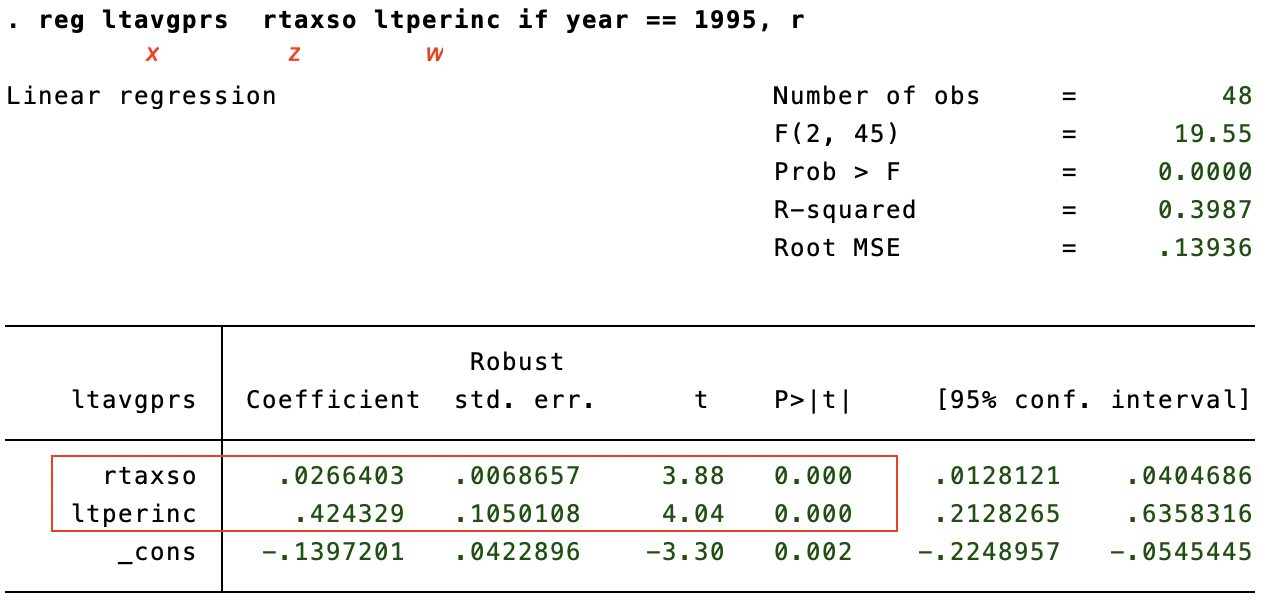
\includegraphics[width=.85\linewidth]{images/2SLS_FS_ols.png}
\end{figure}
\end{frame}

\begin{frame}{Example with $m=1$  -- Price Elasticity of cigarettes}
\begin{figure}
  \centering
         \vspace{-1mm}
         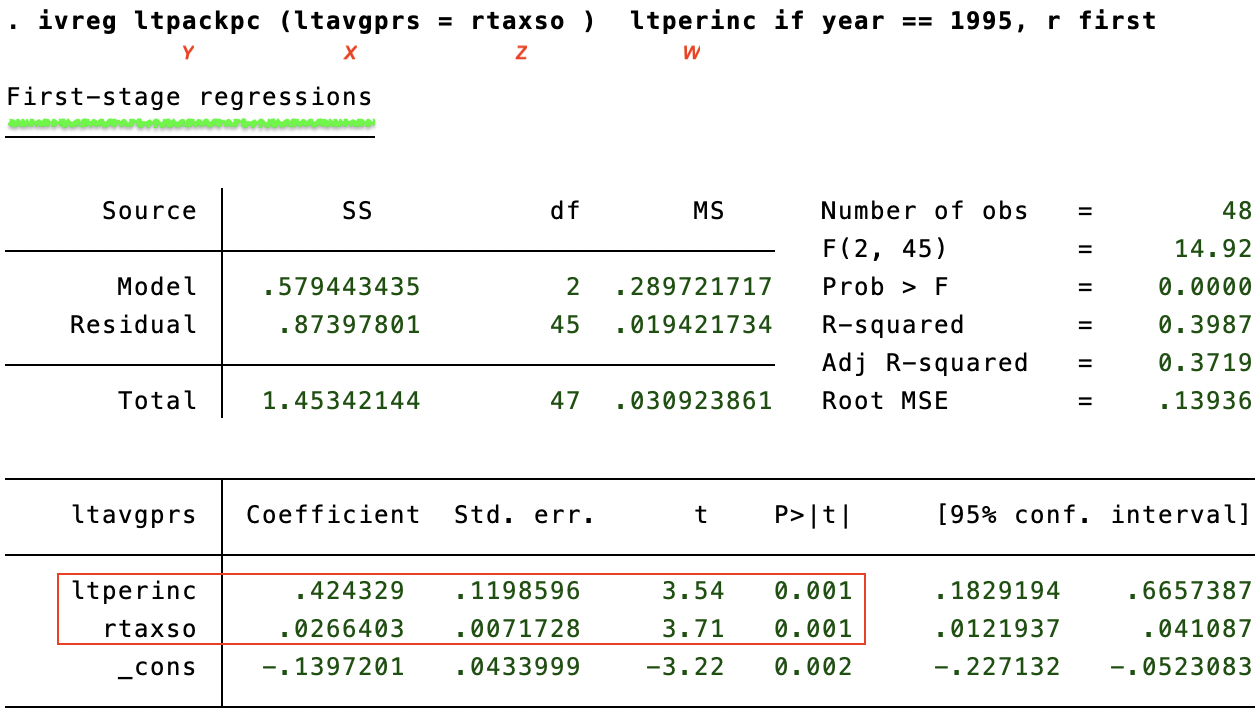
\includegraphics[width=.85\linewidth]{images/2SLS_FS_ivreg.png}
\end{figure}
\end{frame}

\begin{frame}{Example with $m=1$  -- Price Elasticity of cigarettes}
\begin{figure}
  \centering
         \vspace{-1mm}
         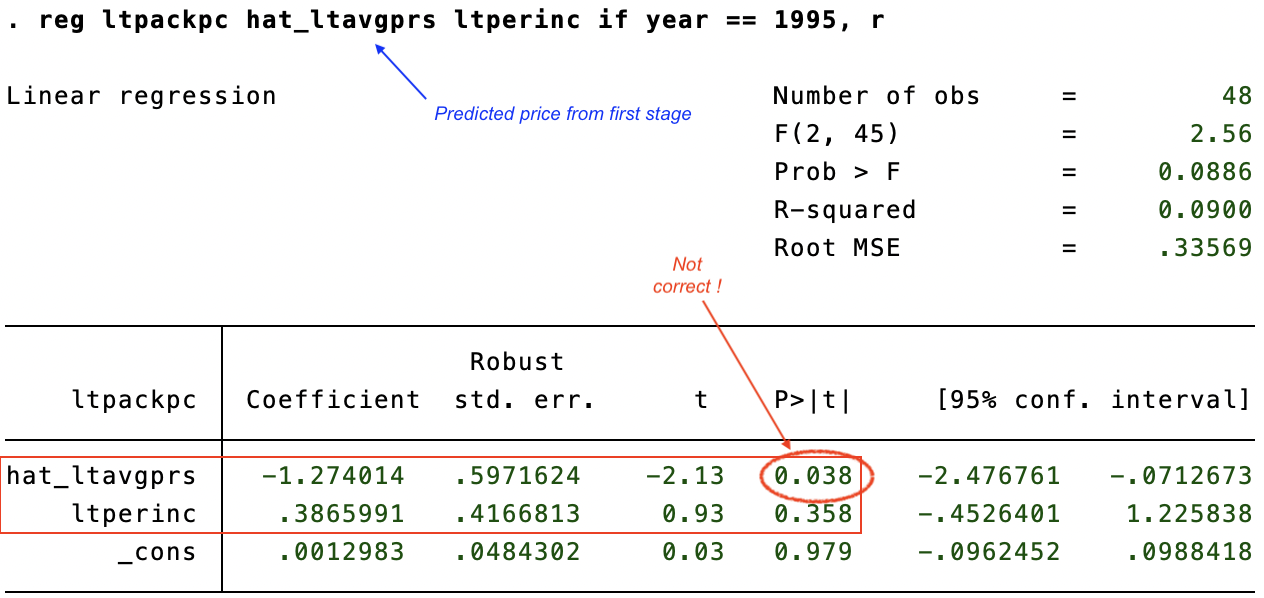
\includegraphics[width=.85\linewidth]{images/2SLS_SS_ols.png}
\end{figure}
\end{frame}


\begin{frame}{Example with $m=1$  -- Price Elasticity of cigarettes}
\begin{figure}
  \centering
         \vspace{-1mm}
         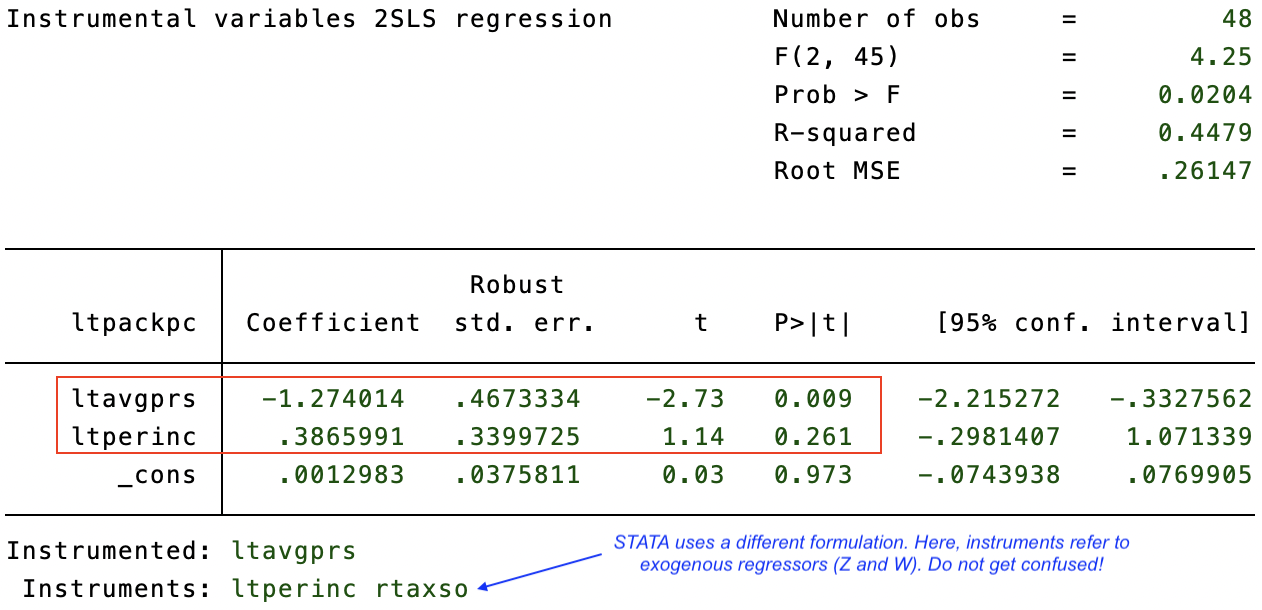
\includegraphics[width=.85\linewidth]{images/2SLS_SS_ivreg.png}
\end{figure}
\end{frame}


\begin{frame}{The General IV Regression Assumptions}
Consider the following specification
\begin{equation*}
    Y_i = \beta_0 + \beta_1 X_{1i} + \dots   \beta_k X_{ki} +  \beta_{k+1} W_{1i} + \dots + \beta_{k+r+1} W_{ri} + u_i
\end{equation*}
and $m$ instruments, $Z_{1i}, \dots,Z_{mi}$. Under the following assumptions, the 2SLS estimator is consistent and has a sampling distribution that, in large samples, is approximately normal
\setbeamertemplate{enumerate items}[default]
\begin{enumerate}
    \item $\mathbb{E}(u_i\mid W_{1i}, \dots, W_{ri}) = 0$ 
    \item $(Y_i, X_{1i},  \dots , X_{ki}, W_{1i}, \dots, W_{ri},Z_{1i}, \dots,Z_{mi})$ are i.i.d.
    \item Large outliers are unlikely: The $X$’s, $W$’s, $Z$’s, and $Y$ have nonzero finite fourth moments;
    \item The instruments $Z_{1i}, \dots,Z_{mi}$ are valid:
    \begin{enumerate}
        \item \textit{Instrument exogeneity:} $corr(Z_{1i}, u_i)=0, \dots, corr(Z_{mi}, u_i)=0$
        \item \textit{Instrument relevance:} Suppose the second stage regression could be run using the predicted values from the \textit{population} first stage regression. Then there is no perfect multicollinearity in this (infeasible) second-stage regression. Intuitively, the instruments must provide enough information about the exogenous movements in these variables to sort out their separate effects on $Y$.
    \end{enumerate}
\end{enumerate}
\end{frame}


\begin{frame}{Checking Assumption 4.1 -- Instrument exogeneity}
\begin{itemize}
    \item Instrument exogeneity: All the instruments are uncorrelated with the error term
    \item In other words, $Z$ can only impact $Y$ \underline{through} $X$
    \item If the instruments are correlated with the error team, the first stage of 2SLS cannot isolate a component of $X$ that is uncorrelated with the error team, so $\hat{X}$ is correlated with $u$ and 2SLS inconsistent.
    \item If there are more instruments than endogenous regressors, it is possible to test -- \underline{partially} -- for instrument exogeneity.
    \item Intuition: Consider the simplest case:
    \begin{equation*}
        Y_i = \beta_0 + \beta_1 X_i + u_i
    \end{equation*}
    Suppose there are two valid instruments: $Z_{1i}$ and $Z_{2i}$, then you can compute two separate 2SLS estimates. If these 2 2SLS estimates are very different from each other, then something must be wrong: one or the other (or both) of the instruments must be invalid
\end{itemize}
\end{frame}

\begin{frame}{Checking Assumption 4.1 -- Instrument exogeneity}
The \textbf{J-test of overidentifying restrictions} (Anderson-Rubin test) makes this comparison in a statistically precise way.\\[1em]

Suppose you have $m>k$. Then,
\begin{enumerate}
    \item Estimate the residuals $\hat{u}^{2SLS}_i$ from
    \begin{equation*}
        Y_i = \beta_0 + \beta_1 X_{1i} + \dots   \beta_k X_{ki} +  \beta_{k+1} W_{1i} + \dots + \beta_{k+r+1} W_{ri} + u_i
    \end{equation*}
    \item Estimate the following model
    \begin{equation*}
        \hat{u}^{2SLS}_i = \gamma_0 + \gamma_1 Z_{1i} + \dots   \gamma_m Z_{mi} +  \gamma_{m+1} W_{1i} + \dots + \gamma_{m+r+1} W_{ri} + e_i
    \end{equation*}
    \item Recover the homoskedasticity-only F-statistic testing $H_0: \gamma_0=\gamma_1=\dots=\gamma_m=0$. The overidentifying restrictions test statistic is $J = mF$
    \item Under the null hypothesis that all the instruments
are exogenous, if $e_i$ is homoskedastic, in large samples $J\sim\chi^2_{m-k}$ where $m-k$ is the degree of \textit{over}identification
\end{enumerate}
\end{frame}


\begin{frame}{Checking Assumption 4.2 -- Instrument Relevance}
In the first stage, we regress
\begin{equation*}
    X_i = \pi_0 + \pi_1 Z_{1i}+ \pi_2 Z_{2i} + \dots + \pi_m Z_{mi} + \pi_{m+1} W_{1i} + \pi_{m+2} W_{2i} + \dots + \pi_{m+k} W_{ki} +u_i
\end{equation*}

The instruments are relevant \underline{\textit{if at least one}} of $\pi_1, \dots, \pi_m$ is non-zero\\

The instruments are said to be \underline{\textit{weak}} if all the $\pi_1, \dots, \pi_m$ are either zero or nearly zero\\[1em]

$\Rightarrow$ \textbf{Weak instruments} explain very little of the variation in $X$, beyond that explained by the $W$’s.\\[1em]

If instruments are weak, the sampling distribution of 2SLS and its t-statistic are not (at all) normal, even with $n$ large.\\[1em]

Remember that $\hat{\beta}_1^{2SLS}= \frac{s_{ZY}}{s_{ZX}} \overset{p}{\to}  \frac{cov(Z_i, Y_i)}{cov(Z_i, X_i)}$ and when instruments are weak, $cov(Z_i, X_i)$ tends to zero...\\[1em]

We cannot conduct statistical inference with the usual methods when instruments are weak (inference under weak instruments is beyond the scope of this course).

\end{frame}



\begin{frame}{Checking Assumption 4.2 -- Instrument Relevance}
\begin{center}
\begin{figure}
    \resizebox{.9\linewidth}{!}{%


\tikzset{every picture/.style={line width=0.75pt}} %set default line width to 0.75pt        

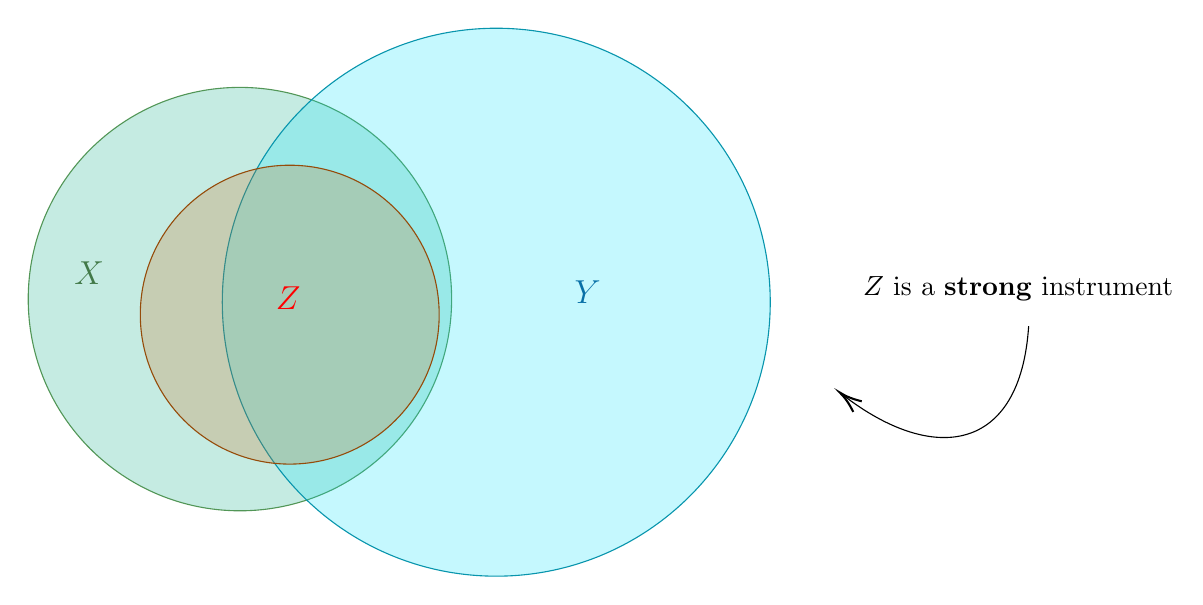
\begin{tikzpicture}[x=0.75pt,y=0.75pt,yscale=-1,xscale=1]
%uncomment if require: \path (0,300); %set diagram left start at 0, and has height of 300

%Shape: Circle [id:dp7275541051674568] 
\draw  [color={rgb, 255:red, 98; green, 178; blue, 9 }  ,draw opacity=1 ][fill={rgb, 255:red, 15; green, 242; blue, 36 }  ,fill opacity=0.24 ] (68,146) .. controls (68,89.67) and (113.67,44) .. (170,44) .. controls (226.33,44) and (272,89.67) .. (272,146) .. controls (272,202.33) and (226.33,248) .. (170,248) .. controls (113.67,248) and (68,202.33) .. (68,146) -- cycle ;
%Shape: Circle [id:dp29955697964696837] 
\draw  [color={rgb, 255:red, 9; green, 107; blue, 178 }  ,draw opacity=1 ][fill={rgb, 255:red, 15; green, 179; blue, 242 }  ,fill opacity=0.24 ] (161.5,147.5) .. controls (161.5,74.6) and (220.6,15.5) .. (293.5,15.5) .. controls (366.4,15.5) and (425.5,74.6) .. (425.5,147.5) .. controls (425.5,220.4) and (366.4,279.5) .. (293.5,279.5) .. controls (220.6,279.5) and (161.5,220.4) .. (161.5,147.5) -- cycle ;
%Shape: Circle [id:dp26088917675528234] 
\draw  [color={rgb, 255:red, 178; green, 9; blue, 9 }  ,draw opacity=1 ][fill={rgb, 255:red, 242; green, 15; blue, 31 }  ,fill opacity=0.24 ] (122,153.5) .. controls (122,113.74) and (154.24,81.5) .. (194,81.5) .. controls (233.76,81.5) and (266,113.74) .. (266,153.5) .. controls (266,193.26) and (233.76,225.5) .. (194,225.5) .. controls (154.24,225.5) and (122,193.26) .. (122,153.5) -- cycle ;
%Curve Lines [id:da7864761338128692] 
\draw    (550,159) .. controls (546.04,220.38) and (503.86,225.89) .. (460.32,192.04) ;
\draw [shift={(459,191)}, rotate = 38.5] [color={rgb, 255:red, 0; green, 0; blue, 0 }  ][line width=0.75]    (10.93,-3.29) .. controls (6.95,-1.4) and (3.31,-0.3) .. (0,0) .. controls (3.31,0.3) and (6.95,1.4) .. (10.93,3.29)   ;

% Text Node
\draw (186,139) node [anchor=north west][inner sep=0.75pt]   [align=left] {\textcolor[rgb]{1,0,0}{{\large $Z$}}};
% Text Node
\draw (330,136) node [anchor=north west][inner sep=0.75pt]  [font=\large,color={rgb, 255:red, 10; green, 6; blue, 235 }  ,opacity=1 ] [align=left] {$Y$};
% Text Node
\draw (89,127) node [anchor=north west][inner sep=0.75pt]  [font=\large,color={rgb, 255:red, 79; green, 139; blue, 13 }  ,opacity=1 ] [align=left] {$X$};
% Text Node
\draw (469,134) node [anchor=north west][inner sep=0.75pt]   [align=left] {$Z$ is a \textbf{strong} instrument};


\end{tikzpicture}
}
\end{figure}
\end{center}

\end{frame}



\begin{frame}{Checking Assumption 4.2 -- Instrument Relevance}
\begin{center}
\begin{figure}
    \resizebox{.9\linewidth}{!}{%


\tikzset{every picture/.style={line width=0.75pt}} %set default line width to 0.75pt        

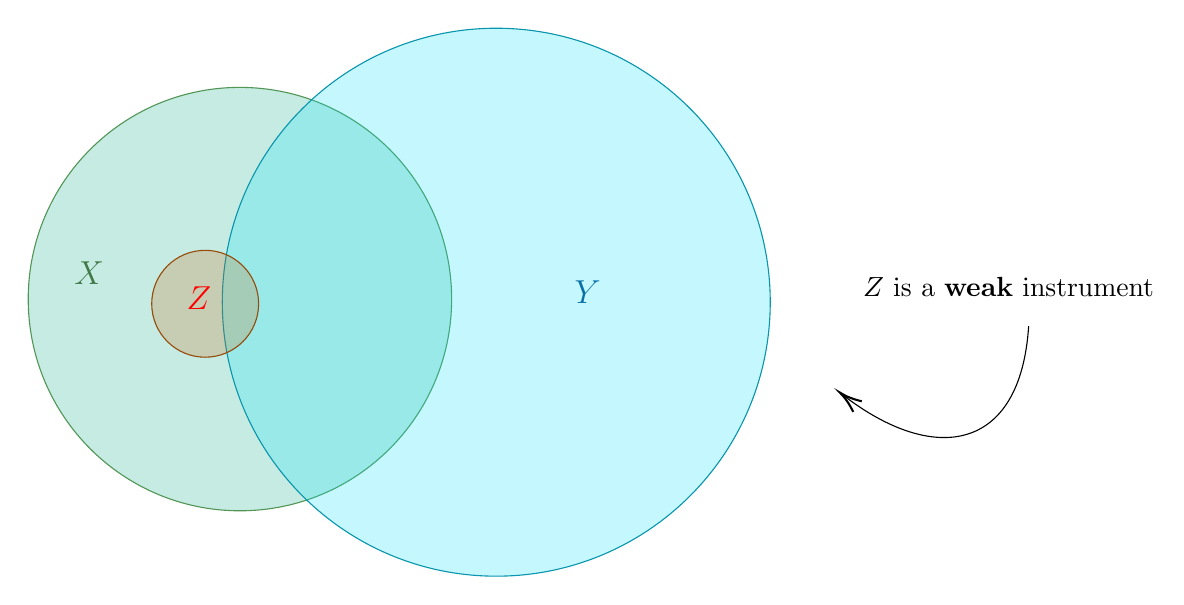
\begin{tikzpicture}[x=0.75pt,y=0.75pt,yscale=-1,xscale=1]
%uncomment if require: \path (0,300); %set diagram left start at 0, and has height of 300

%Shape: Circle [id:dp7275541051674568] 
\draw  [color={rgb, 255:red, 98; green, 178; blue, 9 }  ,draw opacity=1 ][fill={rgb, 255:red, 15; green, 242; blue, 36 }  ,fill opacity=0.24 ] (68,146) .. controls (68,89.67) and (113.67,44) .. (170,44) .. controls (226.33,44) and (272,89.67) .. (272,146) .. controls (272,202.33) and (226.33,248) .. (170,248) .. controls (113.67,248) and (68,202.33) .. (68,146) -- cycle ;
%Shape: Circle [id:dp29955697964696837] 
\draw  [color={rgb, 255:red, 9; green, 107; blue, 178 }  ,draw opacity=1 ][fill={rgb, 255:red, 15; green, 179; blue, 242 }  ,fill opacity=0.24 ] (161.5,147.5) .. controls (161.5,74.6) and (220.6,15.5) .. (293.5,15.5) .. controls (366.4,15.5) and (425.5,74.6) .. (425.5,147.5) .. controls (425.5,220.4) and (366.4,279.5) .. (293.5,279.5) .. controls (220.6,279.5) and (161.5,220.4) .. (161.5,147.5) -- cycle ;
%Shape: Circle [id:dp26088917675528234] 
\draw  [color={rgb, 255:red, 178; green, 9; blue, 9 }  ,draw opacity=1 ][fill={rgb, 255:red, 242; green, 15; blue, 31 }  ,fill opacity=0.24 ] (127.5,148.25) .. controls (127.5,134.03) and (139.03,122.5) .. (153.25,122.5) .. controls (167.47,122.5) and (179,134.03) .. (179,148.25) .. controls (179,162.47) and (167.47,174) .. (153.25,174) .. controls (139.03,174) and (127.5,162.47) .. (127.5,148.25) -- cycle ;
%Curve Lines [id:da7864761338128692] 
\draw    (550,159) .. controls (546.04,220.38) and (503.86,225.89) .. (460.32,192.04) ;
\draw [shift={(459,191)}, rotate = 38.5] [color={rgb, 255:red, 0; green, 0; blue, 0 }  ][line width=0.75]    (10.93,-3.29) .. controls (6.95,-1.4) and (3.31,-0.3) .. (0,0) .. controls (3.31,0.3) and (6.95,1.4) .. (10.93,3.29)   ;

% Text Node
\draw (143,139) node [anchor=north west][inner sep=0.75pt]   [align=left] {\textcolor[rgb]{1,0,0}{{\large $Z$}}};
% Text Node
\draw (330,136) node [anchor=north west][inner sep=0.75pt]  [font=\large,color={rgb, 255:red, 10; green, 6; blue, 235 }  ,opacity=1 ] [align=left] {$Y$};
% Text Node
\draw (89,127) node [anchor=north west][inner sep=0.75pt]  [font=\large,color={rgb, 255:red, 79; green, 139; blue, 13 }  ,opacity=1 ] [align=left] {$X$};
% Text Node
\draw (469,134) node [anchor=north west][inner sep=0.75pt]   [align=left] {$Z$ is a \textbf{weak} instrument};


\end{tikzpicture}
}
\end{figure}
\end{center}

\end{frame}



\begin{frame}{Checking Assumption 4.2 -- Instrument Relevance}
So... how relevant must the instruments be to draw causal inference in practice? How weak is weak?

\begin{itemize}
    \item Staiger and Stock (1997)’s Rule of thumb (1 endogenous variable!): Reject that your instruments are weak if $F\geq10$
    \item Stock and Yogo (2005) formalized and generalized Staiger and Stock (1997) : Reject that your instruments are weak if $F > J_{10}(m)$ where $J_{10}(m)$ is chosen such that $P(F > J_{10}(m) ~~|~~ \text{2SLS bias $\leq$ 10\% $\times$ OLS bias)}= 0.05$

\end{itemize}\\[1em]

The literature on weak instrument testing is still ongoing (technical details are beyond the scope of this class)\\[1em]

So if you have weak instruments,
\begin{itemize}
    \item Get better instruments (often easier said than done!)
    \item If you have many instruments, some are probably weaker than others and it’s a good idea to drop the weaker ones (dropping an irrelevant instrument will increase the first-stage F)
    \item If you only have a few instruments, and all are weak, then you need to switch from 2SLS to a method that is robust to weak instruments.
\end{itemize}
\end{frame}

\begin{frame}{Summary}
\begin{itemize}
    \item A valid instrument lets us isolate a part of $X$ that is uncorrelated with $u$, and that part can be used to estimate the effect of a change in $X$ on $Y$\\[1em]
    \item IV regression hinges on having valid instruments:
    \begin{enumerate}
        \item Exogeneity: Test overidentifying restrictions via the J-statistic + exercise your judgment 
        \item Relevance: Check via first-stage F
    \end{enumerate}\\[1em]
    \item A valid instrument isolates variation in $X$ that is ``as if'' randomly assigned.\\[1em]
    \item The critical requirement of at least $m$ valid instruments cannot be tested -- you must use your head!
\end{itemize}
\end{frame}


\begin{frame}[allowframebreaks]{Material}
\begin{itemize}
    \item[--] \textbf{Textbooks:}
    \begin{itemize}
        \item Introduction to Econometrics, 4th Edition, Global Edition, by Stock and Watson -- Chapters 12 - 13
        \item Introductory Econometrics, 5th Edition, A Modern Approach, by Jeff. Wooldridge -- Chapter 15.
        \item Causal Inference, The Mixtape, by Scott Cunningham -- Chapter 6
    \end{itemize}
    \item[--] \textbf{Papers:}
    \begin{itemize}
        \item Angrist, J. D., \& Krueger, A. B. (1991). Does compulsory school attendance affect schooling and earnings?. The Quarterly Journal of Economics, 106(4), 979-1014.
        \item Hoxby, C. M. (2000). Does competition among public schools benefit students and taxpayers?. American Economic Review, 90(5), 1209-1238.
        \item Gruber, J., \& Hungerman, D. M. (2007). Faith-based charity and crowd-out during the great depression. Journal of Public Economics, 91(5-6), 1043-1069.
    \end{itemize}
\end{itemize}
\scriptsize{
\bibliographystyle{ecta}
\bibliography{base} 
}
\end{frame}


\end{document}



